\documentclass[a4paper, 11pt]{article}
\usepackage[T1]{fontenc}
\usepackage{subfigure}
\usepackage[margin=2.5cm, nohead]{geometry}
\usepackage{palatino, url, multicol}
\usepackage{amssymb, graphicx, fancyhdr, latexsym, url, verbatim}
\usepackage{algorithm, algorithmic}
\usepackage{hyperref}
\usepackage{clrscode3e}
\usepackage[all]{xy}
\usepackage[english]{babel}
\usepackage{matlabScripts}
\usepackage{caption}


\newcommand{\projectName}{ACHTBITS}
\newcommand{\projectAbbreviation}{Awesome
CHaradriiformes Toegepast BIrd Tracking System}
\newcommand{\bits}{BITS}

\addtolength{\footskip}{-90mm}
\addtolength{\headheight}{-05mm}
\addtolength{\headsep}{05mm}

%\pagestyle{fancy}
\lhead{\projectName}
%\chead{Annotation Tool - User Guide}
\rhead{\small \textsc{\projectAbbreviation}}
%\cfoot{\footnotesize \textit{ \projectAbbreviation}\\[0.1cm] \small \thepage}
%\cfoot{}
%\rfoot{\thepage}


\setlength{\parindent}{0pt}
\setlength{\parskip}{10pt}

\begin{document}

\newcommand{\HRule}{\rule{\linewidth}{0.5mm}}

\begin{titlepage}
\begin{center}

\includegraphics[width=1\textwidth]{uva}\\[0.5cm]

\HRule \\[0.2cm]
{ \huge \LARGE \textbf{\projectName}\\[0.1cm]
\large \textsc{\projectAbbreviation}\\[0.15cm]
\Large User Guide
 \vspace{0.2cm}}
\HRule \\[0.4cm]
\Large \today

\vfill

\begin{tabular}{cccc}
Jesse Eisses & Sosha Happel & Maarten Inja & Maarten de Waard \\ 
6352189 & 6273831 & 5872464 & 5894883 
\end{tabular} \\[0.3cm]

\large \{mrtndwrd, maarten.inja, jesse.eisses, soshappel\}@gmail.com 
\end{center}
\end{titlepage}

%%{
%\begin{center}
%% Upper part of the page
%
%\textmd{Leren en Beslissen verslag}
%\vfill
%% Title
%{ \huge \textbf{ACHTBITS} \\\large \textsc{Awesome Charadriiformes Toegepast
%BIrd Tracking System}
%}\\[0.4cm]
%%\begin{center}
%\vfill
%By\\
%\vfill
%%\large\textbf{{Maarten de Waard \\ 5894883},  {Maarten Inja \\ 5872464},  {Jesse Eisses \\
%%6352189}, {Sosha Happel \\ 6273831}}
%\begin{tabular}{cccc}
%Jesse Eisses & Sosha Happel & Maarten Inja & Maarten de Waard \\ 
%6352189 & 6273831 & 5872464 & 5894883 
%\end{tabular}
%\vfill
%\{mrtndwrd, maarten.inja, jesse.eisses, soshappel\}@gmail.com
%%6352189 \and Sosha Happel\\ 6273831}
%\end{center}
%
%\end{titlepage}
%%}

%\thispagestyle{empty}
\vspace*{00mm}
\tableofcontents
\newpage

\section{Overview}
% Overview of the functionality of the tool

This tool was created to aid the annotation of data from the UvA-BITS (BIrd Tracking System) database, in particular data of the lesser black-backed gull above the North sea. The tool contains:
\begin{itemize}
\item
a script that reads raw data downloaded from the database and creates flight-sessions.
\item
an automated segmentation algorithm that splits sessions into clusters that are likely to belong to the same class of behaviours 
\item
a GUI that shows information about a cluster and lets the user choose a behaviour class.
\item
A shell that runs through all sessions of a device and calls the annotation tool
\item
Functions to prepare the annotated data for a classification algorithm
\end{itemize}

\section{Installation}
% short explanation of how to get the tool ready for use
\begin{itemize}
	\item
	download the tool \footnote{\url{http://achtbits.googlecode.com/files/}}
	\item
	extract the zip to a folder (referred to as installFolder)
	\item
	run matlab
	\item
	in matlab, navigate to installFolder/matlab
\end{itemize}
\section{Usage}
\subsection{Downloading \& Preprocessing Data}
% how to get data from the database ready for the tool
\subsubsection{Downloading Data From the Database}
The data we need to use is available from a database at the UvA-bits website
\footnote{\url{https://public.flysafe.sara.nl/phppgadmin/} }. This database is often very slow 
and sometimes overloaded. This is why we downloaded all the data we required in one run. 
Before we can start in \textsc{matlab} we preprocess this data to load only correct data
in it.

The query we use to download the GPS data is of the following format: 

%\lstinputlisting[language=SQL]{queryies.sql}
\begin{verbatim}
select *
from gps.uva_tracking_speed_3d_limited
where device_info_serial = 344 
and date_time > '2008-07-01 00:00:00' 
and date_time < '2012-08-01 00:00:00';

\end{verbatim}

The query we use to download the accelerometer data is of the following format:
\begin{verbatim}
select a.device_info_serial, a.date_time, a.index,
(a.x_acceleration-d.x_o)/d.x_s as x_cal,
(a.y_acceleration-d.y_o)/d.y_s as y_cal,
(a.z_acceleration-d.z_o)/d.z_s as z_cal
from gps.uva_device_limited d
full outer join gps.uva_acceleration_limited a
using (device_info_serial)
where a.device_info_serial = 344 and
a.device_info_serial = d.device_info_serial and
a.date_time > '2008-07-01 00:00:00' and a.date_time < '2012-08-01 00:00:00'
order by a.date_time, a.index;
\end{verbatim}

Only the \textit{device\_id} should change to select different. Obviously more complex queries could 
decrease the magnitude of the task of our preprocessing script but we wanted to keep the
work for the database to a minimum for (reasons discussed earlier) and this seemed the
easiest way to do this. 

The result of the queries should be dumped in one folder to `comma separated files' (csv) files.
The data filenames should be the following : DATA\_ALL\_[GPS/ACCELEROMETER]\_BIRD\_X.csv for 
GPS or accelerometer data for \textit{device\_id} X. 

\subsubsection{Creating Session Files}
Now the data is downloaded it can be preprocessed before \textsc{matlab} can do its magic. 
This can done for a single \textit{device\_id} by \textit{PreprocessCsvFiles.java} or 
for multiple \textit{device\_id}s by \textit{Wrapper.java}. The Wrapper simply uses the PreprocessCsvFiles. 

A special \textit{config.txt} that can be adjusted for those who do not like to program 
Java can be used to customize the script PreprocessCsvFiles. This configuration file
has a couple of lines with description=value. The value (the part after an equal sign)
can be adjusted to whatever legal
value one
would like. The description (the part before an equal sign) can be anything one would
except more equal signs. Do not change the order of the lines.

The only variables that are not self explanatory are those that decide which columns
of the input data file should be used (those columns that should be extracted from the
input files and should be put in the output files). 
This is an array with integers and there are 
two for these, one for the GPS data files and one for the accelerometer data files. 
Luckily, these should not have to be changed since the current values extract all the 
relevant
columns. 

Both scripts work with command line arguments. For more elaboration one what the
scripts exactly do one could check our report for an extensive list or the README file for 
a short overview. 

Command line arguments for PreprocessCsvFiles (do not change the order of these arguments): 
\begin{itemize}
    \item The .csv file with GPS data.
    \item The directory in which to create a folder with the session files.
    \item (Optional argument) The .csv file with accelerometer data.
\end{itemize}

Command line arguments for Wrapper (do not change the order of these arguments): 
\begin{itemize}
    \item The output directory in which to create folders with the sessions.
    \item The input director which contains all the data files (of the known format). 
\end{itemize}


















 
\subsection{Annotating Sessions and Clusters}

The main function to use the annotation tool is annotateBird, this functions takes a deviceId, loops through all sessions in the folder of the device and puts them into the tool. The function is a shell for annotateSession, which runs the tool on one session. When this function is run independently there is no guarantee that the results will be properly saved, so this is not advised. The classes given as user input are added to the features of the cluster and these are saved to a file to a file. For a more detailed explanation, please refer to the help documents of the functions (in matlab enter: help 'functionName')\\ \\
\newpage
{
\begin{figure}[h]
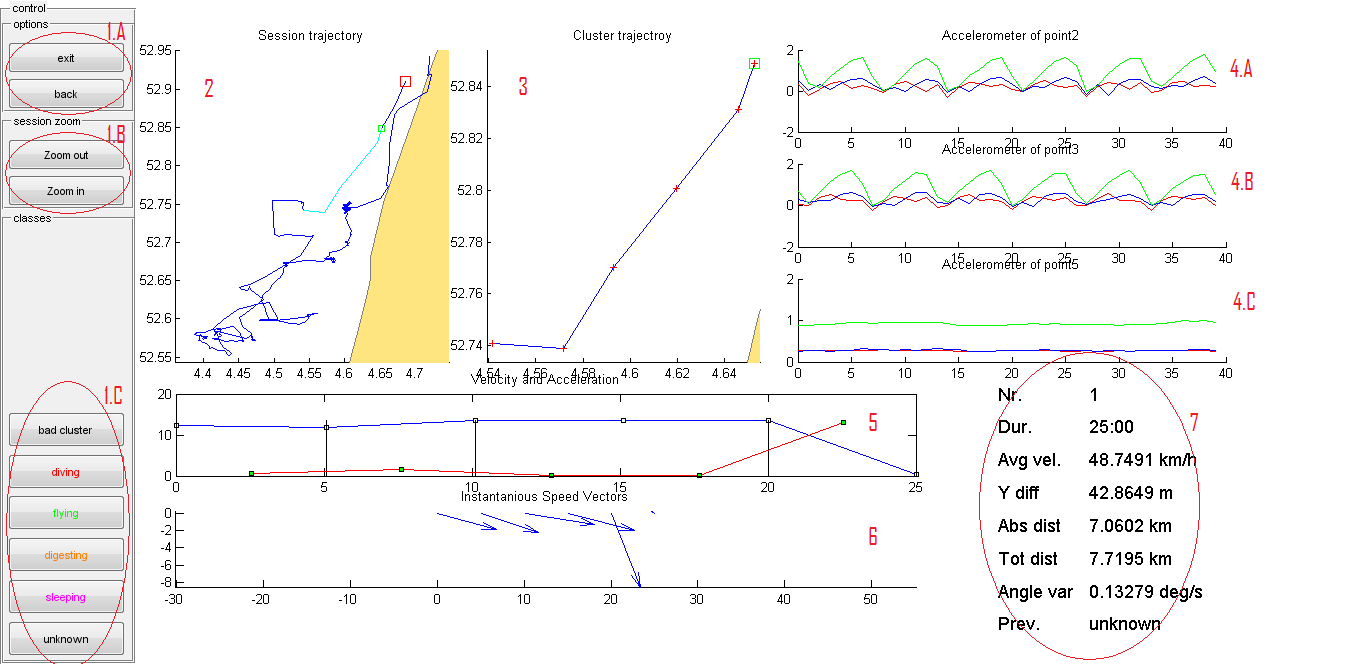
\includegraphics[scale = 0.5]{tool_overview_indexed.png}
\caption{an overview of the layout of the annotation-tool}
\end{figure}
}
Layout:
\begin{enumerate}
	\item button control
	\begin{enumerate}
		\item
		exit - closes the tool\\
		back - returns to the previous cluster
		\item
		zoom in - zooms in on the whole session\\
		zoom out - zooms out to the entire coast of the Netherlands
		\item
		classes - a group of class buttons used to annotate the current cluster
	\end{enumerate}
	\item
	plot of the trajectory of the session\\
	the current cluster is highlighted in light blue\\
	the start of the session is marked with a red square\\
	the start of the current cluster is marked by a green square\\
	the previous clusters are color coded with their class
	\item
	plot of the trajectory of the current cluster\\
	the start of the cluster is marked by a green square
	\item
	accelerometer-data plots of the points marked by a vertical line in the velocity plot
	\item
	velocity and acceleration plot
	\item
	instantaneous speed and direction vectors
	\item
	features of the current cluster
\end{enumerate}
		
 % running and using the tool

\subsection{Using the Resulting Annotated Features}

% what the tool outputs and how this can be adjusted
The tool created a csv file for every annotated session. They are stored in a folder hierarchy in \verb|tools/annotatedData/real/|. To use this data in a learning algorithm you will need one large csv file of cluster features and annotations. The function \verb|createTrainingData.m| does this automatically. You can run it from matlab without any arguments, you only have to navigate to the folder containing the annotated data (\verb|tools/annotatedData/real/| by default). It will output the files \verb|AllFeatures.csv| and \verb|classes.txt|, which maps annotation IDs to strings.
Depending on your machine learning tool you might need to apply some of the following changes in \verb|AllFeatures.csv|:
\begin{itemize}
	\item Replace all $-1$ values with missing values characters ('?' in WEKA)
	\item Replace all class IDs (the last two columns) with strings (\verb|classes.txt| shows which ID belongs to which class)
\end{itemize}

\section{Making Adjustments}
% things that could be added and how this should be done

\subsection{Adding Features}

To add new features you will have to modify the matlab code of the tool. All features generated by the tool are created in \verb|createClusterFeatures.m|, with exception of the \emph{previsousCluster} feature. Any new features can be appended to the return value of this function. 

If you want to add features to already annotated data, you can use the \verb|reloadFeatures.m| function. This script basically recreates all clusters and features from the raw data, and transfers the \emph{annotation} and \emph{previousCluster} columns from the already annotated data. After executing the function you must navigate to your annotated data folder in the dialog (\verb|tools/annotatedData/real/| by default). Inside this directory a new folder is created called \verb|real_reloaded|, containing the new features (this can take a few minutes). The raw device data should be located in \verb|tools/parsedCsvFiles/| for this to work.

\end{document}
